\documentclass[a4paper,12pt]{article}
\renewcommand{\baselinestretch}{1.5}

\usepackage[english]{babel}

\usepackage{graphicx}
\usepackage{tikz}
\usetikzlibrary{positioning}
\usepackage{pgfplots, pgfplotstable}
\pgfplotsset{compat=1.8}

\usepackage{natbib}
\usepackage{tipa}
\usepackage[font={small,it}]{caption}
\usepackage[titletoc,title]{appendix}

\graphicspath{ {./images/} }
\DeclareCaptionFont{tiny}{\tiny}

\title{Mechanical Turkish}

\author{ Veltzer Doron\\
Department of Linguistics\\
Tel Aviv University\\
Ramat Aviv, Tel Aviv, \underline{Israel} }
\date{\today}

\begin{document}
\maketitle

\begin{abstract}
This paper proposes Recursive Neural Networks (RNNs) as phonological models. In order to demonstrate
their effectiveness I revisit \cite{becker_phonological_2009} (and \cite{becker_surfeit_2011})
summarize it's OT account of Turkish's stem final voicing alternations and criticize it on the
grounds of implausible learnability, I then show how RNN structure based models would handle the
same phenomenon in a simpler and more learnable manner ending in displaying results of an RNN topology
used to model the phenomenon tracing its development motivation to such innate facts as the temporal
nature of speech and the articulator.
\end{abstract}

% table of contents
\pagebreak
\tableofcontents

% Start the actual paper on a new page.
\pagebreak
\section{'Surfeit of the stimulus' revisited}

Turkish is an SOV agglutinative Altaic language that has come a long way from the Mongolian steppes,
in it's passage it has come into extensive language contact with dominant representatives of two
other language families, namely Persian (IE) and Arabic (Semitic).

The agglutinative nature of Turkish means that suffixes are omnipresent and morpho-phonological
phenomena centers around the points of agglutination, here I survey one of the simplest morphemes,
the accusative form, a high vowel (marked I) suffix under-specified for back and round features. The
flagship of Turkish phonology Vowel Harmony (VH) then causes the suffix to harmonize its missing
features. we disregard VH here and focus instead on the consonants p,t,\textipa{\t{tS}},k at the
endings of stems.

\subsection{The phonetic phenomenon at hand}

The accusative form frequently causes voicing alternation, this has traditionally been analyzed as
final devoicing in the stem's final consonant rather than voicing in the accusative form (in which
case the UR is assumed to be voiced), since we examine the task of deducing the accusative form
given the stem, we follow \cite{becker_surfeit_2011} in disregarding the traditional analysis and
assume the final consonant's unvoiced PR to be the UR input for the accusative form.

The alternation is lexically specified and largely unpredictable environment wise (unless that
environment encompasses the entire stem). Observe the extreme case of examples \textipa{[ama\t{tS}]}
'purpose' \textipa{[ama\t{tS}W]} (+acc) and \textipa{[ana\t{tS}]} 'mother hen'
\textipa{[ana\t{dZ}W]} (+acc). That said, the alternation does however correlate strongly to
certain features of the alternating consonant and its nearby environment.

In \cite{becker_phonological_2009}, results by \cite{moreton_analytic_2008} are reasserted in
Turkish. While inspecting the Turkish lexicon as gleaned from Berkeley's TELL database
(\cite{inkelas_turkish_2000}) correlations between accusative voicing alternation of final
consonants and various environment aspects are found statistically significant \footnote{All of the
following also have non trivial mutual correlations (i.e. in order to predict the probability of
alternation in the lexicon it is beneficial to model all correlating parameters together rather
than one at a time)} and thus predictive of the phenomena:
\begin{itemize}
  \item The stem length greatly increases alternations, three C final stem forms were analyzed,
  CVC, CVCC \& CVCVC, (longer than that the alternation seems to tend to 100\% in an oscillating
  manner).
  \item The Point Of Articulation (POA) of the alternating consonant affects alternations forming a
  U shape as a function of backwardness.
  \item High vowels preceding alternating consonants increase alternations.
  \item Back vowels preceding alternating consonants increase alternations.
  \item Voice for preceding consonants do not have any significant effect.
\end{itemize}
In order to examine these in terms of speaker productivity Istanbul Turkish speakers were asked to
apply the accusative form to nonce words, the results showed that speakers had productive knowledge
as to the mutual correlations of length and POA effects (figure \ref{fig:lenPOA}), but little to no
(to opposite) knowledge with respect to qualities of the preceding vowel (figures \ref{fig:height}
\& \ref{fig:backness}).
\begin{figure}[!ht]
\centering
\includegraphics[width=0.85\textwidth]{lenPOA.eps}
\caption{Speaker production rates plotted and regressed against tendencies in the lexicon. Data
points relate to stem length and alternating consonants POA.}
\label{fig:lenPOA}
\end{figure}
\begin{figure}[!ht]
\centering
\begin{minipage}[b]{0.45\textwidth}
\centering
\includegraphics[width=0.85\textwidth]{height.eps}
\captionsetup{font=tiny}
\caption{Speaker alternation differences between ±high preceding vowels plotted and regressed
against tendencies in the lexicon. Different data points relate to stem length and alternating
consonant's POA.}
\label{fig:height}
\end{minipage}\hfill
\begin{minipage}[b]{0.45\textwidth}
\centering
\includegraphics[width=0.85\textwidth]{backness.eps}
\captionsetup{font=tiny}
\caption{Speaker alternation differences between ±back preceding vowels plotted and regressed
against tendencies in the lexicon. Different data points relate to stem length and alternating
consonant's POA.}
\label{fig:backness}
\end{minipage}
\end{figure}

This result is in line with cross linguistic universal language tendencies. Length and POA effects
are prevalent across many languages whereas vowel quality effects are extremely rare. In those rare
cases where languages exhibit effects of preceding vowel quality it is usually attributed to
perception and has a reversed correlation trend to the one present in the Turkish lexicon.

Existence of the trend itself is attributed to Arabic loan words as \cite{becker_phonological_2009}
explains: ``In Turkish borrowings of words with voiced stops in the source language, final
devoicing in the bare stem but not in the forms with vowel-initial suffixes causes nouns to become
alternating (e.g. Arabic bur\textipa{dZ} 'sign' > Turkish bur\textipa{tS} bur\textipa{dZ}u),
whereas source words that end in a voiceless stop don't alternate across the paradigm. Arabic lacks
the consonants [p] and \textipa{[\t{tS}]} and has many nouns that end in [b] and \textipa{[\t{dZ}]},
and as consequence the lexicon’s overall alternation rates are boosted for those places of
articulation. On the other hand, the existence of many Arabic nouns with feminine suffix -at/-et
boosted the number of non-alternating, non-high vowel, coronal-final nouns. Ultimately, however, the historical
explanation for these lexical trends is obviously completely inaccessible to speakers who are not
experts in historical linguistics.''

\subsection{Analysis within OT}
\cite{becker_phonological_2009} then offers an OT model for this seemingly selective statistical
learning phenomenon by making use of the mechanisms of Constraint Cloning (CC) and Recursive
Constraint Demotion (RCD). Briefly, CC operates so that whenever learners detect a grammar conflict
between a pair of surface forms they clone the constraint that caused the conflict (choosing which
constraint to clone is somewhat more complicated than might appear at first glance, for details
see \cite{pater_locus_2007}). After cloning, the two constraints subdivide the lexicon between them
with indexed UR relating the stem to it's delegated constraints, this is repeated until the
behavior of speakers is modeled. I assume the reader to be acquainted with RCD (for details see
\cite{tesar_multi_recursive_1997}).

The relevant OT constraints cloned in this analysis are \textsc{Ident}(voice) and \textsc{Max}
producing 2 clones for each combination of the examined stem length and POA, i.e. 2*3*4 constraints
that partition the lexicon.

The unlearned relatedness to preceding vowel quality is explained away on the other hand by simply
claiming no markedness constraints exist to correlate preceding vowel quality and voicing
(${*V_{[+HIGH]}C_{[+VOICE]}}$ or ${*V_{[+BACK]}C_{[+VOICE]}}$), not allowing learners to learn such
correlations.

The work ends by reasserting that when exposed to the lexicon a general statistical learner, such as
the Minimal Generalization Learner (MGL) whose results are presented, will learn all available
correlations including the surfeit and in doing so will greedily overshoot the mark and
``outperform'' native speakers\footnote{This in turn is used to suggest that speakers are not full
statistical learners but rather learn correlations when those are in line with UG}.

\subsection{Critique}
First for a trite. In the vowel quality height production test (figure \ref{fig:height}) it is
claimed that the [\textipa{tS}] and [p] consonants cannot be considered outliers since they include
too many of the alternations, that however does not deny the possibility that their behaviors are
the results of a different strata at work \footnote{The outlier comment was made in the first place
since with these points removed a near perfect 1-1 regression line would be made quite apparently}.
As stated, both these consonants usually originate stem finally from Arabic load words,
additional evidence for the operation of a second strata in Arabic loan words can be found in
the fact that Arabic loan words often do not comply with VH and are easily identifiable by
speakers\footnote{It remains to be lamented that this phase of the experiment not carried out using
 child speakers (as were all other following parts of the experiment) since it would have
ascertained if less knowledge of word origin produces more production errors.}.

This critique doesn't hold for the backwardness test (figure \ref{fig:backness}) since that test
clearly demonstrates no speaker reproduction ability. For the sake of simplicity, from now on, I
follow Becker in claiming that no speaker reproduction of preceding vowel quality effects exist.

The second point to be raised is a much more problematic one, namely, that of learnability. How can
one entertain the learning process involved in a constraint cloning process? How can the speaker
hold several simultaneous constraint EVAL derivations when the production mechanism itself is
singular? Such a double learning mechanism would require at least some form of neural structure
cloning which is extremely unlikely, How can the speaker then compare the two derivations side by
side and detect the correct cause of the conflict? (remembering that this is not at all a trivial
process). This follows explanations of variation (such as \cite{coetzee_phonological_2008}) in
positing the ability of an online learning process to keep two derivations side by side, but
whereas those presuppose an inner homunculus, CC exaggerates in presupposing a linguistically
inclined inner homunculus complete with pen and paper.

One might claim that this is an OT problem at the edge of phonology and one possible modelling of
it at that but clashes between statistics and UG such as these are omnipresent and the given
explanation is in fact inevitable. As a side note, I'll mention having tried to reformulate this
within OT in a more plausible learnable manner and failed. Furthermore, up to some fundamental
shift in OT I believe an explanation of this sort being inevitable could be formally proven.

One might also claim the model does not pertain to the actual learning or productive process, this
is a claim much harder to rebuke but other problems exist. Out of the overall errors and variations
produced by the two speakers in the 6000 relevant stems in the TELL database 95\% relate to our
phenomena (the other mostly relate to the Arabic originating and much harder to transcribe double
consonants) suggesting extreme learning difficulties even for native speakers in the lexicon
proper, these same speakers exhibit a 94\% agreement on alternations in lexical terms. CC would have
an extremely hard time explaining such errors and productive variations in the lexicon.

In nonce words, speaker agreement is, for obvious reasons, much lower (Pearson r correlation between
two speakers' outputs is bound at about 0.2 with a p value of around 0.7). CCs apply to nonce words
by competing as to which is applied and hence operate with the frequency of their respective
percent of the lexicon. Why then would such a mechanism prove confusing for speakers to use?

Last but not least is the fact that all speakers' nonce productions are lower than the matching
percentage existent in the lexicon and while even child speakers exhibit the correct statistical
patterns these patterns are attenuated so that children produce much less alternations overall than
both adults and lexicon statistics.

All of this begs for an altogether different explanation.

\section{Phonological neural network (NN) modelling}

This paper on the one hand is quite unorthodox in trying to bridge the gap between Computational
Linguistics and Natural Language Processing (NLP) but does not on the other hand have the scope to
go in depth into the topic of Machine Learning (ML) NNs and more specifically deep learning and
Recursive NNs (RNNs). Despite many of these models being initially proposed for and inspired by
phonology they have seen little to no use in modelling it and are instead kept busy producing state
of the art results all across the board in NLP) solving problems higher up in the language tree
from those of morphology to those of sentiment analysis (all having immediate economical applications).

For a quick review of the history of machine learning, see appendix a. For a referential look at
whatever work has been previously done in modelling phonology with NNs see appendix b. I kept the
discourse in these appendices mostly referencial and hopefully in par with the understanding level
of a budding NLP scientist and/or an interested phonological minded computational linguist and will
henceforth limit my NLP outbursts in the work itself to topics directly related to and facilitating
modelling of the phonological Turkish phenomenon.

\subsection{Some technical details}

Perusing the TELL lexicon I first qualitatively reaffirmed all the observations regarding the
correlations. As for speaker productivity, I have not the means to reproduce the nonce word tests
conducted on native Turkish speakers, so, taking these results as given fact all my tests involved
teaching the lexicon to a learning neural net model and examining its effectiveness both in quickly
memorizing the forms recorded in the TELL corpus and in reproducing the nonce accusative form
statistics of Turkish speakers, i.e. reproducing correlations of stem length and POA while ignoring
correlations of preceding Vowel quality.

The most crucial issue in learning is balancing memorization (over-fitting) and generalizing. NNs
are deterministic machines, interestingly enough in ML as opposed to in linguistics variation
is rarely as major a concern as accuracy, noise is thus not typically used to model variation but
rather to force the NN to generalize. The noise levels are set high enough to make it impossible
for the NN to model the noise existing in the data itself (called over-fitting the error signal).
Such noisy models with increased generalization cause quite a counter intuitive speedup in learning
where the size of the learned corpus is rendered quite irrelevant, this is a well known fact in NLP
and was also noticed and mentioned by \cite{boersma_convergence_2008}.

The nonce words for speaker productivity tests were carefully constructed by Turkish phonologists to
``sound'' Turkish, generating a large enough list proved problematic. As a result I had to generate
enough ``speakers'' whose outputs I could average. Since NNs are deterministic machines for
each utilized network topology I computed 100 random weight settings with different random seeds and
the output of these I averaged to compute production statistics.

Since the TELL corpus contains output variation and disagreement between its two speakers (with
agreement measured at about 94\%) I provided the networks with a gold standard goal of around 96\%
accuracy for lexicon learning and removed all variation in the output, leaving a sensible margin so
as not to force too exact a memorization of the data and instead solicit generalizing as much as
possible.

For the networks' input, after culling the overall 6000 possible stems for duplicate forms and
variation I removed all but the CVC, CVCC and CVCVC prosodic structure stems studied in the
article, the final input thus consisted of a collection of 854 stem forms. Once these were set I
used what is called a one hot representation, where each input phoneme is given as a long vector
(with one dimension per language phoneme) with its proprietary dimension coordinate set to 1. The
phonemes then enter an embedding layer which translates them to certain representations found
beneficial by the network's learning process for modelling the input to output mapping.

The output had two distinct setups described further on.

All models were built trained and tested using \cite{chollet_keras_2015} (under
\cite{theano_development_team_theano_2016}).
\footnote{Not having the breadth necessary to fully disclose all NN modelling and results I instead
verbally detail all results that promote the goal of relating the development process that went into
engineering the topology of the network and will present only the results for the final structure,
however, all csv data used for input \& output as well as the full training and testing scripts and
all results can be found at https://github.com/veltzerdoron/Mekanichal-Turkish}

\subsection{Weakening NNs powers of generalization}

NNs are as a whole generalizing machines and given sufficient neurons and structural connectivity
will approximate any mapping. In ML, weakening a model's powers of generalization is, as far as I
know, never an issue.

\subsubsection{Experiment 1: deep NN modelling}

Output of the following two experiments is a single bit denoting the alternation of the input stem.

First I let an NN with enough neurons arranged in multiple layers learn the alternation, the middle
layers of such NNs are called hidden and the NNs themselves are dubbed deep NNs. These deep
networks' learning process allow each of their neurons to deduce their local constraints in order
to solve the global mapping problem induced by the given input output pairs.

The goal in this experiment was to show that such an NN would learn the lexicon and reproduce all
existent statistical correlations but in fact for reasons explained further on, the NN never
generalized well enough and instead simply memorized the lexicon, so that when it achieved the
required 96\% accuracy it processed nonce words in patterns that bared little resemblance to those
produced by speakers.

\subsubsection{Experiment 2: Simple RNN modelling}

Next I shifted the network's topology into the time dimension by using an RNN structure, RNNs differ
from NN models in that each layer projects not only to the next layer but also to itself in the
next time phase (here, the next phoneme's processing step). This sort of network topology should
echo in the mind of a phonologist structures and notions of auto-segmental phonology.

The serial time shift dramatically changed the probability distribution of the output and took care
of two crucial points in the modelling:
\begin{itemize}
  \item The strong signal in the output showing the importance of length for prediction meant that
  the RNN would model it automatically.
  \item By questioning the model only as to its last output, the network will put a strong attention
  emphasis\footnote{A related problem that might arise from this emphasis is the possibility of it
  expanding to include the immediate environment of the last input, specifically the quality of the
  preceding vowel} on the features of the last input, i.e. the alternating consonant.
\end{itemize}

Results showed that RNNs greatly facilitated learning the alternation as a whole, despite reducing
the number of neurons in the network to a mere 80 they learned the alternations about 20 times
faster than NNs with the same comparative degree of required lexicon accuracy. A strong indication
of generalizing taking place. It took 5 hours to train the required 100 ``speaker'' models.

Examining statistics of output on lexicon stems, despite their being 96\% accurate, the RNNs seemed
to have a comparatively harder time in correlating preceding vowels to alternation than learning the
mutual POA/length correlations. When producing alternation outputs for nonce word this effect seemed
to amplify giving first hints that RNNs was indeed a promising model.

Two other, perhaps related, interesting facts about the nonce word results are the fact that the
entire POA length pattern was attenuated in a manner that placed the RNN model somewhere between
adult and child speakers (and away from lexicon statistics) and the fact that as a whole the
alternation of CVC stems was greatly underestimated.

My hypothesis relating these two facts is that since the lexicon alternation representation is built
bottom up in treelike fashion, the short stems are first learned. Their alternation being as scant
as it is (11\%) allows a learner to entertain a null hypothesis, simply asserting alternations never
occur, has an accuracy of 89\%, with learning and exposure to longer and longer stems (almost always
alternating) this null hypothesis slowly erodes. Null hypotheses are a common issue in ML usually
mitigated by ways such as balancing the examples shown to the network in terms of the output. I
did not test this hypothesis.

\subsubsection{Experiment 3: Final RNN modelling}

There are generally two ways in which a network's generalizing power can be weakened, one way is to
overload its task with other simultaneous tasks, the other is structural modification (for instance
the example we've already seen of using an RNN). The final model combines these two notions.

A network's topology might be altered more in the direction of the desired output if for instance we
would envision a system in which consonant features are processed in a totally separate path from
vowel features such as height and backward positions no interaction could possible ensue
\footnote{This extreme solution would require that the stems be memorized solely in terms
reminiscent of  a root based language like fashion} Although this might work well enough for this
problem it is highly improbable as a solution that could later be extended to other problems.

However, this thought experiment inspires a structural change motivated also by auto-segmental
phonology. As a whole features tend to influence similar features in adjacent phonemes and/or other
features in the same phoneme and to a much lesser extent other features in adjacent phonemes.

\begin{figure}[!ht]
\tikzset{
  every neuron/.style={
    circle,
    draw,
    minimum size = 0.5cm
  },
  neuron missing/.style={
    draw = none, 
    scale = 4,
    text height = 0.333cm,
    execute at begin node = \color{black}$\vdots$
  },
}
\centering
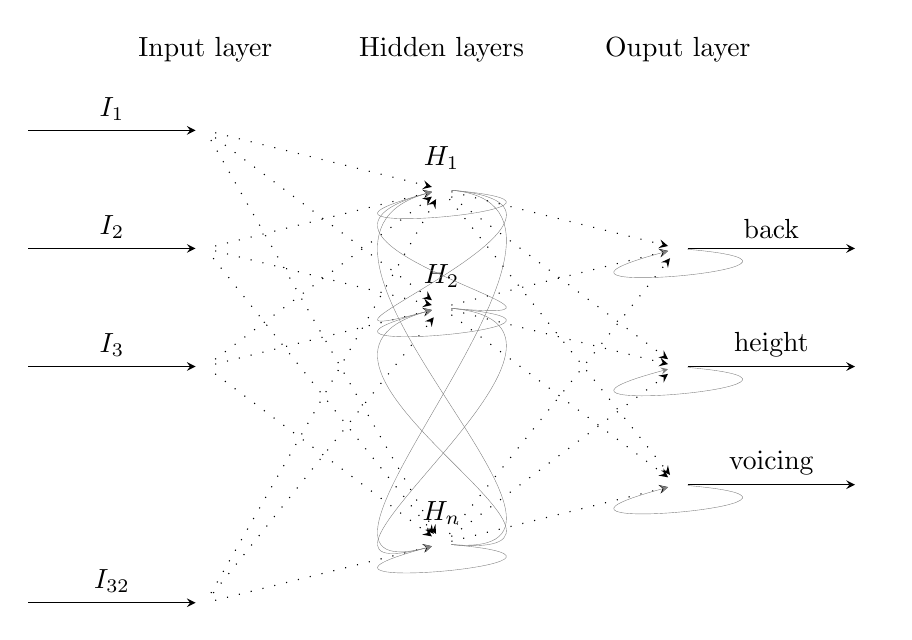
\begin{tikzpicture}[x=1.5cm, y=1.5cm, >=stealth]
\foreach \m/\l [count=\y] in {1,2,3,missing,4}
  \node [every neuron/.try, neuron \m/.try] (input-\m) at (0,2.5-\y) {};
\foreach \m [count=\y] in {1,2,missing,3}
  \node [every neuron/.try, neuron \m/.try ] (hidden-\m) at (2,2-\y*1) {};
\foreach \m [count=\y] in {1,2,3}
  \node [every neuron/.try, neuron \m/.try ] (output-\m) at (4,1.5-\y) {};
\foreach \l [count=\i] in {1,2,3,32}
  \draw [<-] (input-\i) -- ++(-1.5,0)
    node [above, midway] {$I_{\l}$};
\foreach \l [count=\i] in {1,2,n}
  \node [above] at (hidden-\i.north) {$H_\l$};
\foreach \l [count=\i] in {back,height,voicing}
  \draw [->] (output-\i) -- ++(1.5,0)
    node [above, midway] {\l};
% first layer is embedding and not recursive
%\foreach \i in {1,...,4}
%  \foreach \j in {1,2,...,4}
%    \draw [line width=0.05mm,gray,->] (input-\i) to[out=0-5,in=180+25,distance=2.5cm] (input-\j);
\foreach \i in {1,...,4}
  \foreach \j in {1,2,...,3}
    \draw [loosely dotted][->] (input-\i) -- (hidden-\j);
\foreach \i in {1,2,...,3}
  \foreach \j in {1,2,...,3}
    \draw [line width=0.05mm,gray,->] (hidden-\i) to[out=0-5,in=180+15,distance=2.5cm] (hidden-\j);
\foreach \i in {1,2,...,3}
  \foreach \j in {1,2,3}
    \draw [loosely dotted][->] (hidden-\i) -- (output-\j);
\foreach \i in {1,2,3}
  \draw [line width=0.05mm,gray,->] (output-\i) to[out=0-5,in=180+15,distance=2.5cm] (output-\i);
\foreach \l [count=\x from 0] in {Input layer,Hidden layers,Ouput layer}
  \node [align=center, above] at (\x*2,2) {\l};
\end{tikzpicture}
\captionsetup{font=tiny}
\caption{Diagram of the final network topology used. Shown is the input embedding layer with its 32
inputs (1 per Turkish phoneme) and the output layer's 3 neurons with their self recurrent
connectivity and output features (back, height and vocality). Other layers are fully recurrent (all
recursive connections drawn in gray)}
\label{fig:NNdiagram}
\end{figure}

In the proposed model, features start out mixed up in standard phonemic one hot input fashion and
separate while processing takes place till they reach the end of processing and the last layer's 3
neurons, one for each of the output features\ (back, height \& voicing). The output layer's
recursive connections allow each of its neurons to take into account their own output in the previous
time-step and/or the new phonemic input's representation as it is constrained by neurons in
previous layers but not (and this is crucial) the previous time-step output of the other two
feature neurons\footnote{The question whether this loop represents neuronal looping connections in
the actual brain or abstracts a longer loop involving actual audio is left unanswered}. This
causes the correlating of different features across timesteps to become more difficult.

If the outputs of the three neurons were to be seen as representing command lines going to the
articulator organs, this recurrent severing could also be motivated by the fact that the tongue
articulator must have a different command line than that of the vocal folds\footnote{Predicting
a more probable interaction between tongue height and backwardness}

The output of this model was thus changed to include all three output features of the alternating
consonant. For specific feature encodings, results by \cite{stachowski_phonological_2015} were used.
Overloading the task of alternation (or in this case output vocality) prediction with that of
decoding and transmitting as is the back and height features of the input stem's last consonant,
despite being as simple as it is, helps focus height and back features onto their own lines of
control and dissuades the network to a large extent from letting them influence vocality.

\subsubsection{Experiment 3: Results}

For the final model I also increased the number of neurons in the network's hidden layers and
modified the recursive connectivity of the last layer to comply with diagram \ref{fig:NNdiagram}).
Once this was done teaching the network became surprisingly easier and faster than it was to train
the RNN in experiment 2 despite it having less neurons/parameters and its task being a proper subset
of this network's task. Training the 100 required final ``speaker'' models took about 4 hours.

Following are the results of our modified RNNs averaged and split into categories according to
POA and length as they compare both to lexicon statistics and to Turkish speaker production
\footnote{speaker productions were missing for stems of CVCC structure}.

\begin{figure}
\begin{tabular}{l|l|llll}
\multicolumn{2}{l|}{syl \& cons}&RNN&Lexicon&Child&Adult\\
\hline
CVC&k           &3.00\% &4.84\% &0.00\% &3.00\% \\
   &\textipa{tS}&20.00\%&24.24\%&3.00\% &28.00\%\\
   &t           &0.00\% &7.81\% &7.00\% &6.00\% \\
   &p           &43.00\%&37.50\%&17.00\%&34.00\%\\
\hline
CVCC&k           &26.00\%&11.11\%&&\\
    &\textipa{tS}&53.00\%&75.61\%&&\\
    &t           &42.00\%&27.87\%&&\\
    &p           &99.00\%&85.71\%&&\\
\hline
CVCVC&k           &100.00\%&94.71\%&60.00\%&95.00\%\\
     &\textipa{tS}&84.00\% &81.67\%&40.00\%&53.00\%\\
     &t           &25.00\% &31.01\%&10.00\%&31.00\%\\
     &p           &99.00\% &97.37\%&20.00\%&53.00\%\\
\end{tabular}
\end{figure}

The first thing to note is that the RNN has greatly ``outperformed'' native speakers in producing
the mutual pattern for length and POA. A 2nd thing worth mentioning is that alternation are still
slightly underestimated with overall alternations standing at 43\% instead of the lexicon's 52\%,
reasons for this were hinted at in experiment 2.

Lets take a look now at alternation differences as a function of differences in back and height
features of the preceding vowel. As illustrated in \ref{fig:HeightRNNLex} and \ref{fig:BackRNNLex}
we see that the tendency between the lexicon and our models seems to be reversed (as is the case for
native speakers), however, the numbers themselves seem to me quite arbitrary and I would rather
than say the model managed to mimic speaker behavior I will be more careful and say that once
previous vowel quality was barred from affecting alternation it became a variable free to be moved
around by the other requirements from the network, especially since the truly divergent
values where achieved for the consonants with a smaller number of input output stems. Perhaps if one
was to overload the network with a more tasking goal such as modelling the phonemes for the entire
output word and with more input/output pairs a result such as true speaker behaviour could be hoped
for.

\begin{figure}[!ht]
\begin{minipage}[b]{0.45\textwidth}
\centering
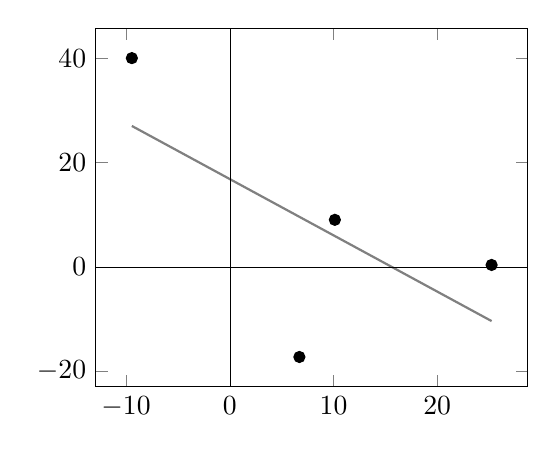
\begin{tikzpicture}
\pgfplotstableread{
  Lexicon RNN
  10.13 9.00
  -9.44 40.00
  25.24 0.35
  6.71 -17.29
}\Height
\begin{axis}[scale=0.8,legend pos=outer north east]
\addplot [only marks, mark = *] table {\Height};
\addplot [thick, gray] table[
    y={create col/linear regression={y=RNN}}
] % compute a linear regression from the input table
{\Height};
\draw[ultra thin] (axis cs:\pgfkeysvalueof{/pgfplots/xmin},0) -- (axis cs:\pgfkeysvalueof{/pgfplots/xmax},0);
\draw[ultra thin] (axis cs:0,\pgfkeysvalueof{/pgfplots/ymin}) -- (axis cs:0,\pgfkeysvalueof{/pgfplots/ymax});
\end{axis}
\end{tikzpicture}
\captionsetup{font=tiny}
\caption{RNN alternation differences between ±high preceding vowels, plotted as a function of
alternating consonant's POA and regressed against lexicon tendencies.}
\label{fig:HeightRNNLex}
\end{minipage}\hfill
\begin{minipage}[b]{0.45\textwidth}
\centering
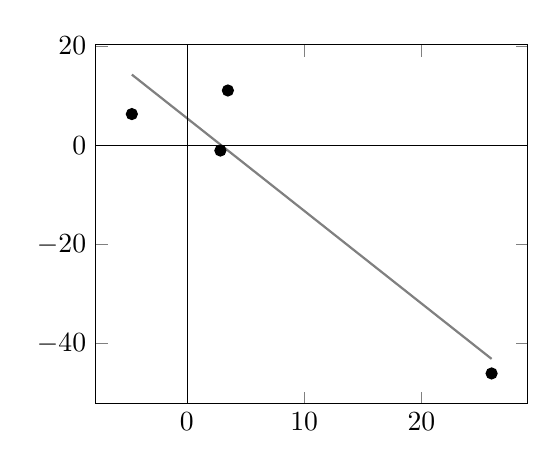
\begin{tikzpicture}
\pgfplotstableread{
  Lexicon RNN
  3.50 11.00
  25.99 -46.00
  2.86 -1.10
  -4.69 6.25
}\Back
\begin{axis}[scale=0.8, legend pos=outer north east]
\addplot [only marks, mark = *] table {\Back};
\addplot [thick, gray] table[
    y={create col/linear regression={y=RNN}}
] % compute a linear regression from the input table
{\Back};
\draw[ultra thin] (axis cs:\pgfkeysvalueof{/pgfplots/xmin},0) -- (axis cs:\pgfkeysvalueof{/pgfplots/xmax},0);
\draw[ultra thin] (axis cs:0,\pgfkeysvalueof{/pgfplots/ymin}) -- (axis cs:0,\pgfkeysvalueof{/pgfplots/ymax});
\end{axis}
\end{tikzpicture}
\centering
\captionsetup{font=tiny}
\caption{RNN alternation differences between ±back preceding vowels plotted and regressed
against tendencies in the lexicon. Different points relate to alternating consonant's POA.}
\label{fig:BackRNNLex}
\end{minipage}
\end{figure}

The given results do, however show that the final structure did achieve at least the goal of
decoupling the influence of preceding vowel quality on alternation.

For completeness I also tried to teach the alternations to a network with the three neuron layer at
its output layer without modifying its recursive connectivity, this structure created a bottleneck
of three dimensional representation and prevented learning altogether, indeed, it proved impossible
to raise the network to the required accuracy no matter how the previous layers were boosted or how
long training took place.

\section{Conclusion}

The paper has shown how a phenomena involving an amalgamation of statistical and universal behaviors
can be effectively modeled step by step by using contemporary learning models such as RNNs. Starting with
a model that performed general statistical learning and gradually working the universal limits
into it by various methods. The actual engineering process involved many more experiments that
proved to be dead ends and were thus not detailed here and yet the path finally followed has a
compelling direct reasoning to it. Conveying the flavor of this sort of reasoning was a major goal
in writing this work.

% Start the appendices on a new page.
\pagebreak

\appendix

\section{Appendix A - On the history of Machine Learning (ML)}

OT arose in the same years perceptron model (first proposed in \cite{rosenblatt_perceptron_1958}) based
structures held sway in ML. Care, must be taken in order to avoid following the induced mixup in
terms, the term constraints in OT parallels what are called features in the perceptron model. The
term features was perhaps at the time taken up by phonological features. I took some care in using
the terms constraints and features as they are used in phonology. Otherwise, from a strictly
functional point of view, the similarity is uncanny.

Whether or not this resemblance is incidental or a result of the supportive theories arising in
similar universities at the same time is besides the point, the farther OT went along in
establishing itself as the go to phonological model, the more similar it became to the perceptron
model, this culminates in proofs for convergence of OT learners where an explicit reference to the
proof being a reformulation of the perceptron convergence theorem is freely made by
\cite{boersma_convergence_2008}.

Two points caused the downfall of perceptron based learning and the beginning of the last AI winter
starting with the end of the peak interest in Neural Networks (NNs) in the early 90s.

First, a simple proof made it abundantly clear that even basic functions such as an exclusive or
(XOR) were unseparable and thus uncalculable by the model, such unseparable functions need to be
encoded in the constraints themselves. This point, however, has no real relevance to OT since the
term constraints itself implies that there is no case where a XOR function needs to be computed
since violating two constraints always outweighs violating each of the constraints separately.

The second point, which is much more damning for OT, is that the resulting system is engineered
rather then learned in the sense that constraints need to be precomputed and not derived by the ML
system on its own. This engineered nature of the model has profound implications, it is not in
itself a problem in case you assume innateness of the constraints in linguistics, or if you are
trying to solve highly human engineered problems in Natural Language Processing (NLP) such as SPAM
detection (a practical field where the perceptron model is still in play) but it is a problem if
innateness is to be exchanged with universality or if an unsupervised ML solution is essential.

\title{Deep networks as automatic learners of constraints}

NNs can be seen as a natural solution when taking the perceptron model and applying it to a general
problem of mapping inputs to outputs. A NN is composed of several connected neurons arranged in
layers with each learning its weights when calculating its relative error in light of solving a
general input to output mapping problem. Countless various algorithms exist and are applied for
more effective learning with most deriving their basic notions from the Back Propagation (BP)
algorithm developed during many years (famously in \cite{rumelhart_learning_1988}).

In cases where there are more than one layer of neurons (as was the case in the perceptron model)
the networks are referred to as deep NNs and all layers not at the input or output layers are called
hidden layers. The hidden layers are seen as freely searching which constraints are worthwhile to
compute locally in order to best model the mapping function.

While writing this, deep NNs are probably the most actively studied topic in the world, it is highly
pertinent both for applications in computer vision and in Natural Language Processing (NLP) and
questions such as how engineered perceptron constraints are embodied in deep networks when they
approach the same problem, how one is to engineer a network's topology and how are the learned
constraints mapped back onto the input level are on the agendas of both technological giants and
academia luminaries.

\subsection{RNNs as a model for finding structure in time}

Recursive NNs (RNNs) are NNs that have backward projecting connections, i.e. networks where
production involves connections from neurons further down the production line back to previous
neurons or to themselves at a later time phase. Both testing and training such networks proceeds
through a simulation of time phases and uses a process called Back Propagation Through Time (BPTT)
reportedly developed independently three times (for instance by \cite{mozer_focused_1989}).

If a network is to predict the next phoneme in language modelling each neuron receives the last
produced output in time and the set of features for the next phoneme and weighs both to produce the
output for the next time sequence and so forth.

As early as they were introduced in \cite{elman_finding_1990} and \cite{jordan_serial_1986} RNNs
seemed to be the correct way to represent the phonological serial to parallel to serial schisms the
brain seems to solve in its processing of time serialized phonetics. Due to technical problems,
this model was buried during the last AI winter and only resurfaced in full force when applied to
economically motivated NLP problems higher up the language tree such as parsing, POS tagging,
pragmatics and Sentiment Analysis (SA).

In all these fields more complex approaches such as bi directional LSTMs based on RNNs (but with
added capability to hold memory for longer time periods) currently produce state of the art
results. Recently some attempts have been made to apply LSTMs to lower levels of the language tree
such as morphology for instance where a bi directional LSTM was taught to predict all morphological
forms of ten languages). LSTM models, however, despite being much more effective than simple RNNs
lack any remote biological precedent.

\subsection{On the psychology of the phonologist \& economics}

Why then would such a model inspire OT as a model for phonology? Perhaps it was exactly its
simplified and engineered nature which allowed it to become a useful tool in the hands of
phonologists who were in turn surprised by such a simple first order approximation being more or
less sufficient for explaining previously unexplained phenomena. For instance one clearly sees
that the closer OT returns to its weighted ancestor the less clear its insightfulness and
manipulability becomes.

A model's manipulability by phonologists and the understandability of its nature, useful as it may
seem, cannot pose a criterion for validity. In the same way the economical applications of a system
should not prove a significant dint in its academic usefulness.

Another explanation for the success of OT might lie in the fact that OT abides so well with the
phonologist's intuitions themselves. In the same manner that the perceptron model is a perfect metaphor
for the consciously mind when it contemplates possibile choice inputs from such unconscious parts of
the mind as are the speech mechanisms, OT can provide a similar metaphor for the phonologist's
conscious mind when it observes phonological phenomena and informs phonological action through the
interaction between the conscious and subconscious parts of the brain by weighing constraints.

Phonology is probably the most subconscious (and thus the most mathematical) of all fields of
linguistic inquiry. It does not have the same subversive effects of conscious attention emphasis
pragmatics or even grammar has, as a result it should have went the same way the visual cortex went
by having its function be the first to be successfully modelled using NNs. The fact that this was
not the case could probably be explained by the fact that tasks such as sentiment analysis were found
much more lucrative.

NLP being largely text oriented and audio applications being so mathematical in nature little
treatment of the intervening space which is Phonology has peaked the interest of technological
companies outside of academia. TTS \& STT applications on the other hand seem as a whole inclined
sadly to ignore this immense field of knowledge. Thus phonology, despite being the original
inspiration for the RNN model, has seen very few attempts throughout the years of RNN modelling.

\section{Appendix B - Previous uses of NNs to model phonology}

The few attempts that have been made to inquire into phonology using NNs as models, some of the
prominent of which made oddly and luckily enough at modelling Turkish phonology, are as a whole
incredibly instructive. The reason for Turkish being so prominent in these attempts becomes clear
when we consider that other attempts involve modelling such languages as Hungarian. Apparently there
is something inherent in VH languages which yields to a computational analysis

\cite{rodd_recurrent_1997}, for instance, built a language model of Turkish words where an RNN was
tasked with the language modelling task of predicting the next phoneme, his attempts involved
creating a bottleneck of representation in the middle hidden layer, starting at a two neuron
bottleneck and moving up to five neurons. his two neuron setup learned the most prominent
alternating regularity of any language, i.e. the regular alternation of consonants and vowels. When
the hidden layer reached four neurons the network showed that it could produced regularities that
exhibited some powers of Vowel Harmony alternation prediction, above that size the networks' outputs
and behaviors were rendered quite uninterpretable (as they eventually always tend to do).

\cite{stachowski_phonological_2015} developed a specific way to encode Turkish phonemes for
application in general NN representation and showed that it improved on previous encoding s when
used to model the Turkish language, I scavenged this paper for some valuable bits of knowledge I used in
the last modeling experiment.

A more theoretical basic approach was taken by \cite{boersma_neural_2013} in modelling the even
lower phonetics of category creation, Boersma used a Boltzmann machine based bi directional
clamping neural structure to show how categories could emerge by teaching it to relate audio
signals and phonemic categories.

\iffalse

\section {Appendix C - Theoretical considerations}

\subsection{Learning issues}

dropout

\subsection{OT NNs and Turing Machines}

In \cite{blutner_neural_2009} fascinating theoretical proofs are built to show that 3 theoreticals
models of computation are reducible and those translatable to one another, these models are OT
constraints Neural Networks and Penalty Logic, these unfortunately have no practical applications as
the reductions could possibly explode as would happen if for instance one would try to formulate
relate weighted non universal constraints and Turing machines.

TODO : mention super turing machines and NNs


\subsection{Future modeling with RNNs}

Ever since Chomsky deriving his inspirations from physical notions of cause and effect, predictive
powers of grammars have always been preferred over cognitive plausibility of the production
process, but predictive powers can be overstated and when the number of prophets grows
exponentially many false ones will undoubtedly predict yet unseen facts truthfully.

Instead of building a phonological model from the bottom up and expecting the existing blocks to
fit previously unencountered phenomena, this paper offers quite a different basic approach
altogether, proposing to add innately motivated constraints onto a full statistical mechanism while
retaining the plausibility of its cognitive base.

Other notions, both those inherited from generative grammar and developed in OT can be abandoned
when direct modelling of corpora is concerned including:
\begin{itemize}
  \item Treating the input as whole words, instead a layered approach where each layer handles a
  distinct phonological level of representation (such as feature, phoneme, syllable, foot, etc\ldots) could
  easily be envisioned.
  \item Generative notions of universality and innateness reinstating themselves in universality of
  the set of OT constraints can easily be replaced with those of learning behaviours inherent in
  neural structures.
  \item The dichotomy of lexicon and production.
  \item The schism between production and modelling.
  \item The implausible and incalculable notion of GEN.
\end{itemize}

Keeping a close relatedness to the perceptron model on the other hand should ensure most OT
explanatory achievements are relatively easily translatable into RNN models as low hanging fruit.

\fi

% Start the references on a new page.
\pagebreak

\bibliographystyle{apalike}
\nocite{*}
\bibliography{Paper}

\end{document}